\section{Pr\'esentation des r\'eseaux de neurones artificiels}

	\subsection{Origine}

Ce sont les neurologues Warren McCulloch et Walter Pitts qui les premiers publi\`erent des travaux sur les r\'eseaux de neurones \`a la fin des ann\'ees 1950. Un mod\`ele simplifi\'e est alors introduit, avec la notion de neurone formel. Le neurone somme ses entr\'ees (avec des coefficients synaptiques) et r\'epond si la somme r\'esultante est sup\'erieur \`a un seuil. Ces r\'eseaux de neurones peuvent th\'eoriquement r\'ealiser des fonctions logiques, arithm\'etiques et symboliques complexes. N\'eanmoins, ces travaux ne pr\'ecisent pas comment faire \'evoluer ces coefficients.

C'est le physiologiste Donal Hebb qui donna un d\'ebut de r\'eponse concernant la modification des coefficients synaptiques. Hebb d\'ecrit en 1949 une r\`egle simple qui permet de modifier la valeur des coefficents synaptiques en fonction de l'activit\'e des unit\'es qu'ils relient.

En 1957, Franck Rosenblatt d\'ecrit le mod\`ele du perceptron. C'est le premier syst\`eme artificiel capable d'apprendre par exp\'erience, m\^eme si des erreurs sont commises. En 1969, Marvin Lee Minsky et Seymour Papert publi\`erent un ouvrage montrant l'impossibilit\'e de traiter des probl\`emes non lin\'eaires avec de tels r\'eseaux. L'industrie s'en d\'etourna et la recherche perdit une grande partie de ses financements.

En 1986, c'est le mod\`ele du Perceptron Multi-Couche, propos\'e par Werbos, Rumerhart et Yann le Cun ind\'ependamment. Ces syst\`emes reposent sur la r\'etropropagation de l'erreur. Ils permettent de traiter avec succ\`es des ph\'enom\`enes non-lin\'eaires.

	\subsection{Utilit\'e}

Les domaines d'applications sont notamment :
\begin{itemize}
	\item classification d'esp\`eces animales par analyse ADN,
	\item reconnaissance de motif (notamment de caract\`eres : OCR),
	\item approximation d'une fonction inconnue, mod\'elisation acc\'el\'er\'ee d'une fonction connue,
	\item estimation boursi\`ere,
	\item m\'et\'eorologie.
\end{itemize}

	\subsection{Principe de fonctionnement}

		\subsubsection{Structure du r\'eseau}

Un r\'eseau de neurone est compos\'e d'une succession de couches dont chacune prend ses entr\'ees sur les sorties de la couche pr\'ec\'edente.

\begin{figure}[H]
	\centering
	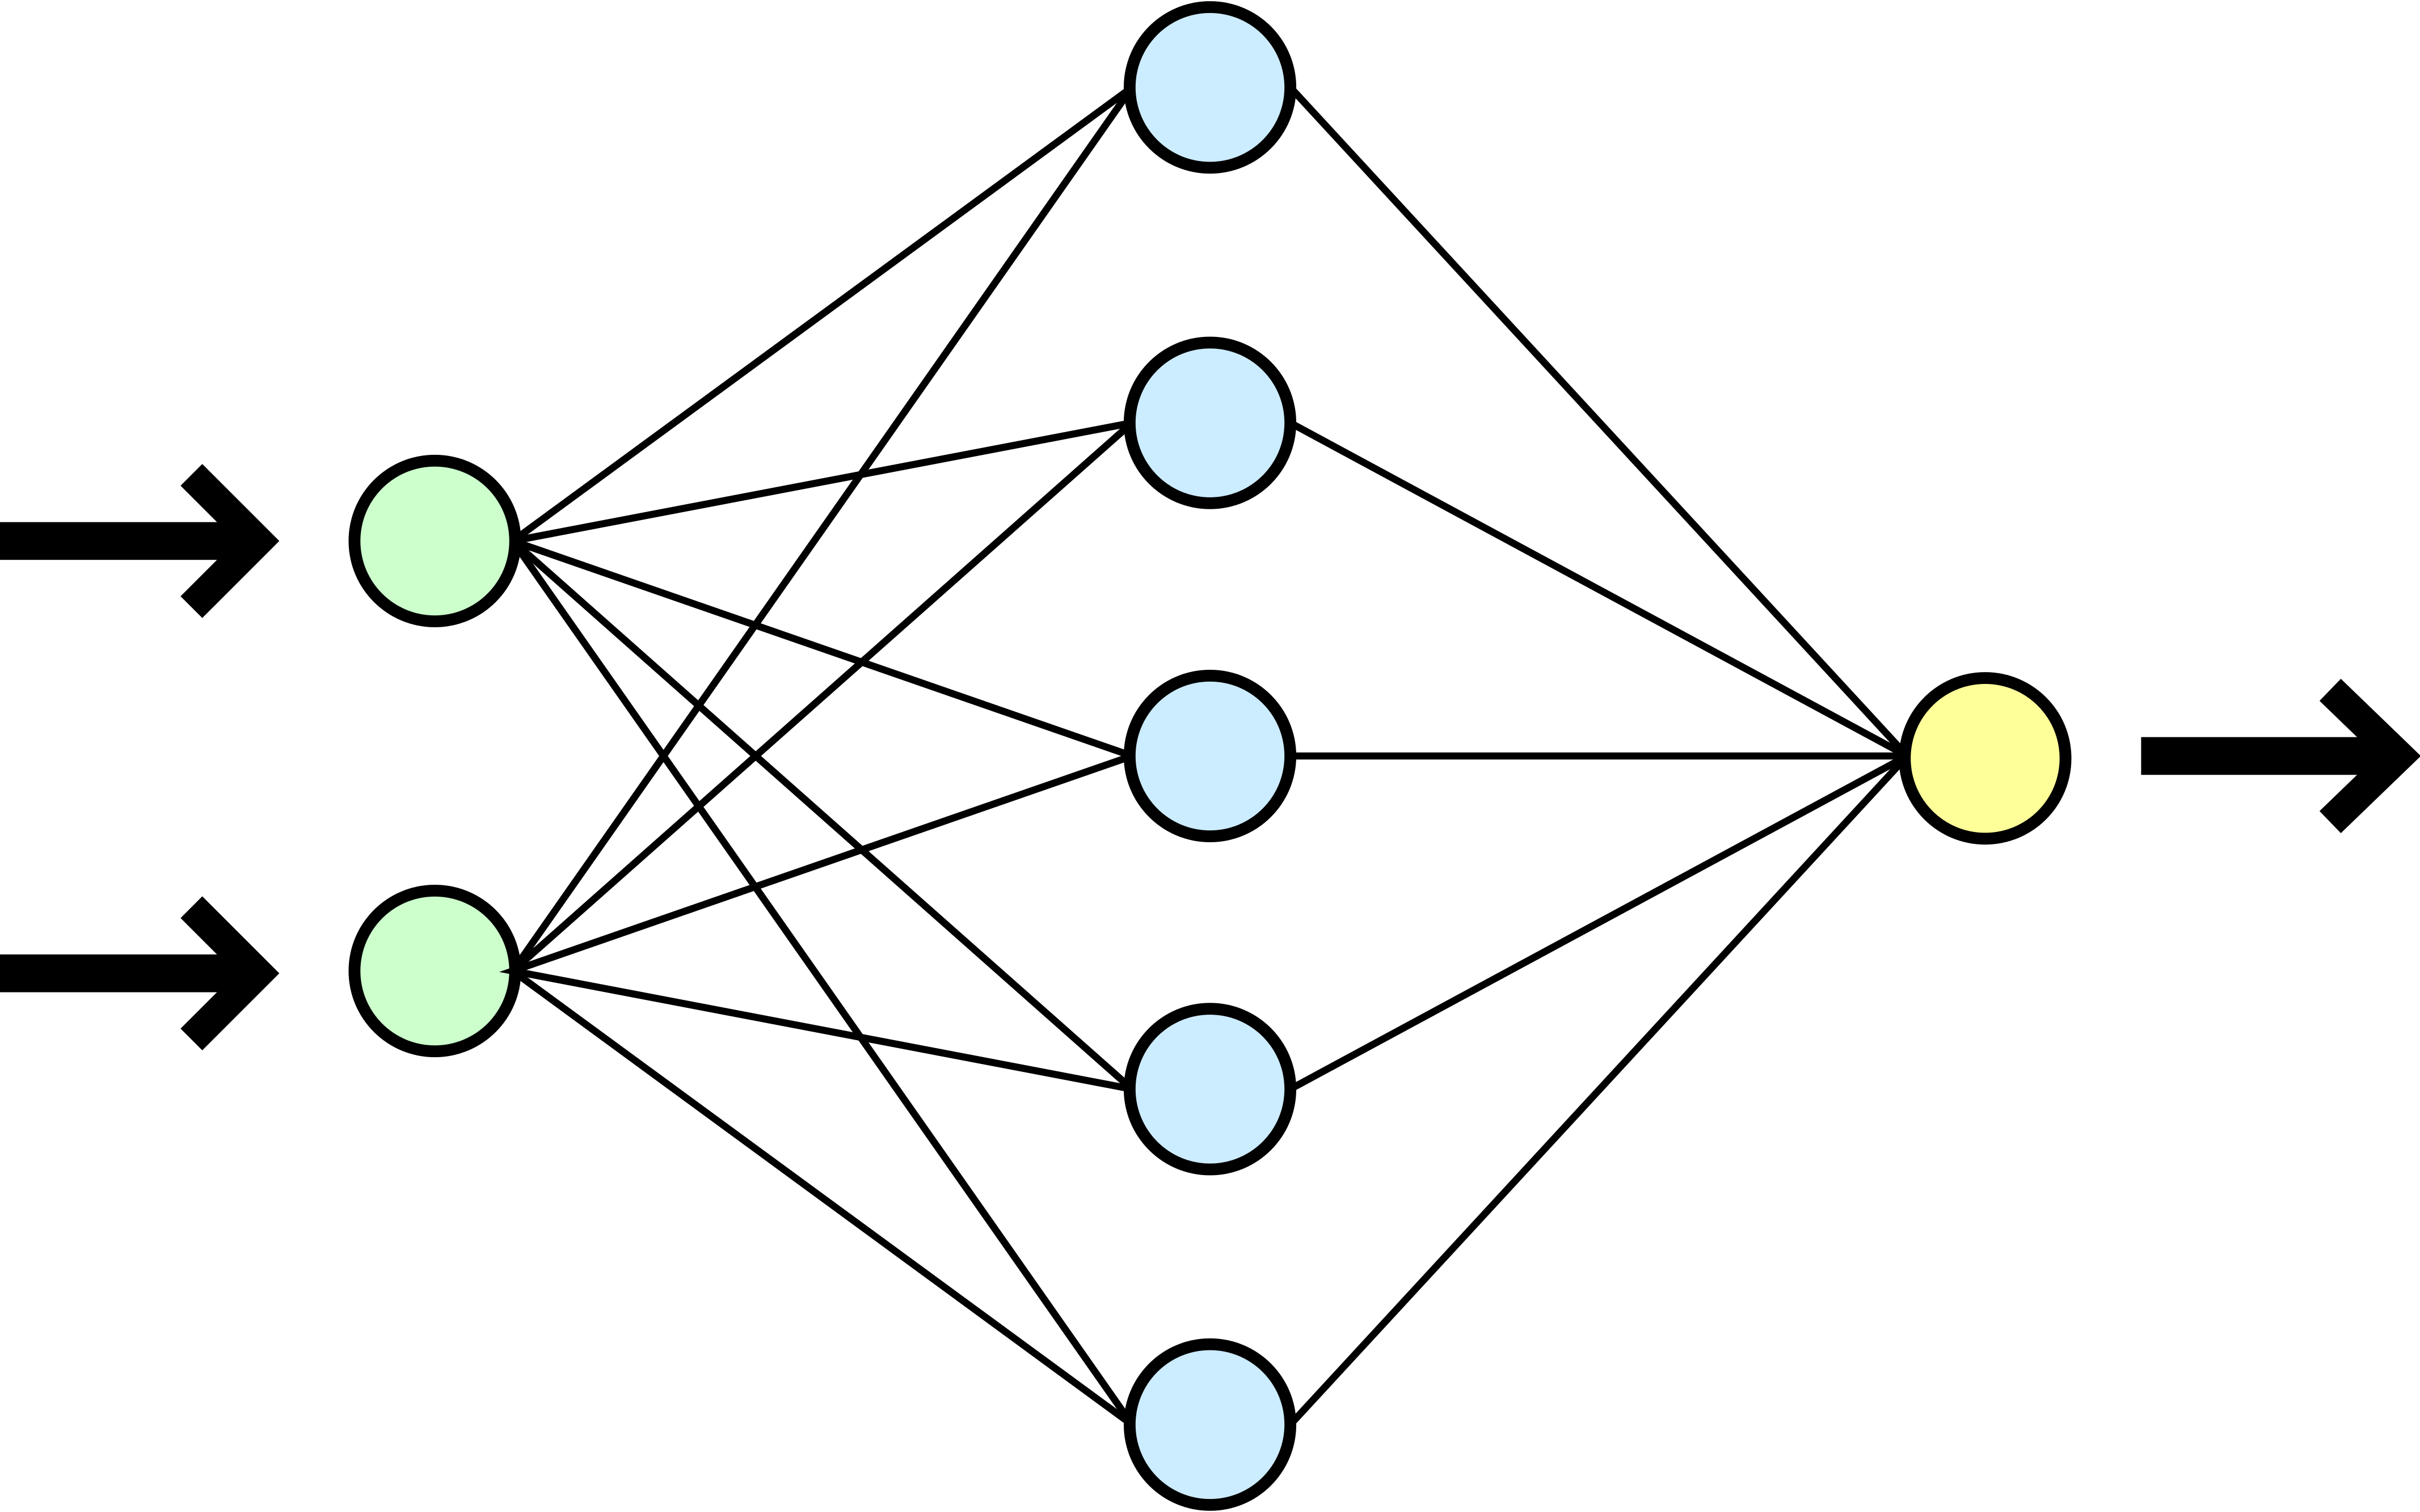
\includegraphics[width=0.66\linewidth]{img/Neural_network.png} 
	\caption{Exemple d'un r\'eseau de neurones avec deux entr\'ees.}
	\label{neurone_ex}
\end{figure}

		\subsubsection{Calcul de la sortie}

\begin{figure}[H]
	\centering
	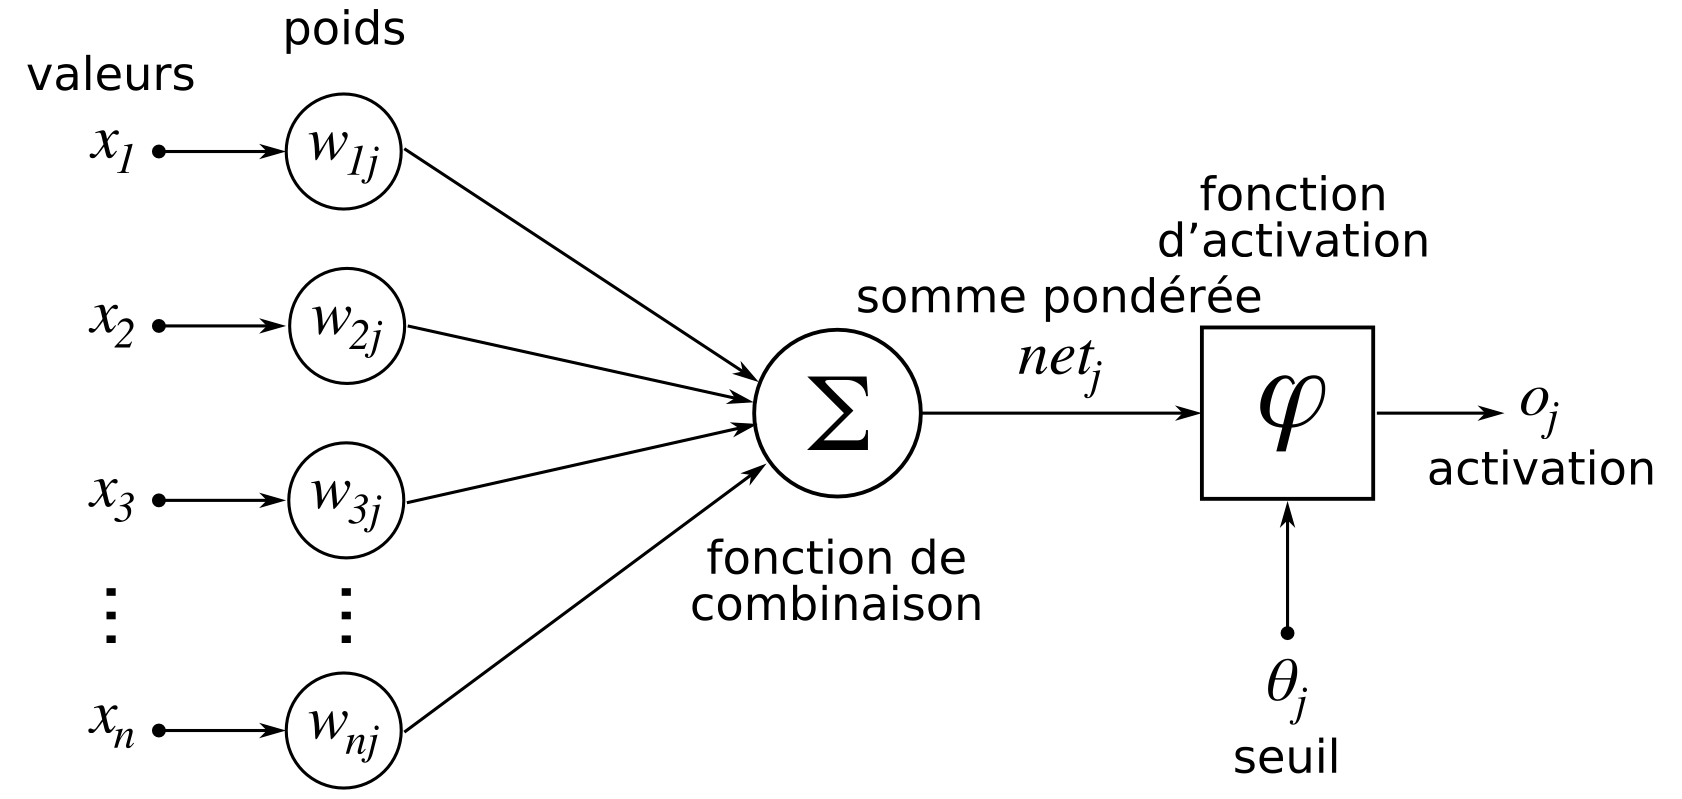
\includegraphics[width=0.66\linewidth]{img/NeuronModel.png} 
	\caption{Fonctionnement sch\'ematique d'un neurone artificiel.}
	\label{neurone_schema}
\end{figure}

Le calcul de la sortie s'effectue selon le sch\'ema explicatif de la figure \ref{neurone_schema}.

		\subsubsection{Fonction de combinaison}

La fonction de combinaison, $\Sigma : \mathbb{R}^n \rightarrow \mathbb{R}$, re\c coit en amont un certain nombre de valeurs via ses connexions synaptiques et retourne un scalaire suivant deux principaux paradigmes :
\begin{itemize}
	\item une combinaison lin\'eaire des entr\'ees (r\'eseaux de type Multi-Layer Perceptron) : $\Sigma(x) = (x,w)$,
	\item la distance entre les entr\'ees (r\'eseaux de type Radial Basis Function).
\end{itemize}

		\subsubsection{Fonction d'activation}

La fonction d'activation sert \`a introduire une non-lin\'earit\'e dans le fonctionnement du reurone. Les fonctions pr\'esentent g\'eneralement trois intervalles :
\begin{itemize}
	\item en dessous du seuil, le neurone est non-actif (sortie \`a $0$ ou $-1$),
	\item aux alentours du seuil, une phase de transition,
	\item au dessus du seuil, le neurone est actif (sortie \`a $1$).
\end{itemize}

Des fonctions classiques de fonctions d'activations sont :
\begin{itemize}
	\item la fonction sigmo\"ide : $f(x)=\frac{1}{1+e^{-\lambda x}}$,
	\item la fonction tangente hyperbolique : $th(x)=\frac{e^x-e^{-x}}{e^x+e^{-x}}$,
	\item la fonction de Heaviside $H(x)=\left\{\begin{matrix} 0 & \mathrm{si} & x < 0 \\ 1 & \mathrm{si} & x \ge 0 \end{matrix}\right.$
\end{itemize}

	\subsection{Apprentissage}

L'apprentissage impliqu\'e dans ces r\'eseaux appartiennent \`a la famille des apprentissages supervis\'es : afin d'amener le r\'eseau \`a avoir le comportement que l'on souhaite, on indique des directions pour am\'eliorer le r\'eseau en donnant des exemples pour lesquels on conna\^it la r\'eponse souhait\'ee.

Un algorithme tr\`es utilis\'e dans ce type d'apprentissages est la r\'etropropagation du gradient (ou encore en anglais backpropagation). Il a pour but de converger de mani\`ere it\'erative vers une configuration optimis\'ee des poids synaptiques.

Soit une entr\'ee $\vec{x}$ et le r\'esultat attendu $\vec{t}$. On propage le signal (gr\^ace \`a la fonction d'activation $g$ et la fonction d'agr\'egation $h$) jusqu'au r\'esultat $\vec{y}$. Pour chaque neurone $i$ dans la couche de sortie, on calcule :
$$e_i^{(s)}=g'(h^{(s)})(t_i-y_i)$$

On propage l'erreur vers l'arri\`ere $e_i^{(n)} \mapsto e_j^{(n-1)}$ gr\^ace \`a la formule suivante :
$$e_j^{(n-1)} = g'^{(n-1)}(h_j^{(n-1)})\sum_i w_{ij}e_i^{(n)}$$

On note :
$$e_j^{(n)} = \sum_i [t_i - y_i] \frac{\partial y_i}{\partial h_j^{(n)}}$$

Enfin, on met \`a jour les poids synaptiques $w_{ij}$ dans toutes les couches :
$$\Delta w_{ij}^{(n)} = \lambda e_i^{(n)}x_j^{(n-1)}$$

o\`u $\lambda$ repr\'esente le taux d'apprentissage (de faible magnitude et inf\'erieur \`a $1$).